% Options for packages loaded elsewhere
\PassOptionsToPackage{unicode}{hyperref}
\PassOptionsToPackage{hyphens}{url}
\PassOptionsToPackage{dvipsnames,svgnames,x11names}{xcolor}
\documentclass[
]{article}
\usepackage{xcolor}
\usepackage[margin = 0.5in]{geometry}
\usepackage{amsmath,amssymb}
\setcounter{secnumdepth}{-\maxdimen} % remove section numbering
\usepackage{iftex}
\ifPDFTeX
  \usepackage[T1]{fontenc}
  \usepackage[utf8]{inputenc}
  \usepackage{textcomp} % provide euro and other symbols
\else % if luatex or xetex
  \usepackage{unicode-math} % this also loads fontspec
  \defaultfontfeatures{Scale=MatchLowercase}
  \defaultfontfeatures[\rmfamily]{Ligatures=TeX,Scale=1}
\fi
\usepackage{lmodern}
\ifPDFTeX\else
  % xetex/luatex font selection
\fi
% Use upquote if available, for straight quotes in verbatim environments
\IfFileExists{upquote.sty}{\usepackage{upquote}}{}
\IfFileExists{microtype.sty}{% use microtype if available
  \usepackage[]{microtype}
  \UseMicrotypeSet[protrusion]{basicmath} % disable protrusion for tt fonts
}{}
\makeatletter
\@ifundefined{KOMAClassName}{% if non-KOMA class
  \IfFileExists{parskip.sty}{%
    \usepackage{parskip}
  }{% else
    \setlength{\parindent}{0pt}
    \setlength{\parskip}{6pt plus 2pt minus 1pt}}
}{% if KOMA class
  \KOMAoptions{parskip=half}}
\makeatother
\usepackage{graphicx}
\makeatletter
\newsavebox\pandoc@box
\newcommand*\pandocbounded[1]{% scales image to fit in text height/width
  \sbox\pandoc@box{#1}%
  \Gscale@div\@tempa{\textheight}{\dimexpr\ht\pandoc@box+\dp\pandoc@box\relax}%
  \Gscale@div\@tempb{\linewidth}{\wd\pandoc@box}%
  \ifdim\@tempb\p@<\@tempa\p@\let\@tempa\@tempb\fi% select the smaller of both
  \ifdim\@tempa\p@<\p@\scalebox{\@tempa}{\usebox\pandoc@box}%
  \else\usebox{\pandoc@box}%
  \fi%
}
% Set default figure placement to htbp
\def\fps@figure{htbp}
\makeatother
\setlength{\emergencystretch}{3em} % prevent overfull lines
\providecommand{\tightlist}{%
  \setlength{\itemsep}{0pt}\setlength{\parskip}{0pt}}
\usepackage{color}
\usepackage{framed}
\setlength{\fboxsep}{.8em}

\usepackage{tcolorbox}

\tcbset{
  mystyle/.style={
    before skip=-10pt, % Adjust this value
    after skip=-10pt   % Adjust this value
  }
}
\newtcolorbox{mynoteblock}[1][]{mystyle, #1}

\newtcolorbox{blackbox}{
  colback=black,
  colframe=orange,
  coltext=white,
  boxsep=5pt,
  arc=4pt}
  
\newtcolorbox{ltbluebox}{
  colback=blue!5!white,
  colframe=blue!75!black,
  boxsep=5pt,
  arc=4pt}
  
\newtcolorbox{ltgreenbox}{
  colback=green!5!white,
  colframe=blue!75!black,
  boxsep=5pt,
  arc=4pt}
  
\newtcolorbox{ltpurplebox}{
  colback=purple!5!white,
  colframe=blue!75!black,
  boxsep=5pt,
  arc=4pt}
  


\newenvironment{cols}[1][]{}{}

\newenvironment{col}[1]{\begin{minipage}[t]{#1}\ignorespaces\vspace{0pt}}{%
\end{minipage}
\ifhmode\unskip\fi
\aftergroup\useignorespacesandallpars}

\def\useignorespacesandallpars#1\ignorespaces\fi{%
#1\fi\ignorespacesandallpars}

\makeatletter
\def\ignorespacesandallpars{%
  \@ifnextchar\par
    {\expandafter\ignorespacesandallpars\@gobble}%
    {}%
}
\makeatother

\usepackage{awesomebox}
\setlength{\aweboxvskip}{1mm}


\pagenumbering{gobble}

\usepackage{enumitem}
\setlist{itemsep=1pt, parsep=0pt} %# Adjust vertical spacing
\setlist[itemize,1]{leftmargin=*, labelsep=0.3em} %# Adjust horizontal spacing
\setlist[enumerate,1]{leftmargin=*, labelsep=0.3em} %# Adjust horizontal spacing

\usepackage{multirow}
\usepackage{multicol}
\usepackage{colortbl}
\usepackage{hhline}
\newlength\Oldarrayrulewidth
\newlength\Oldtabcolsep
\usepackage{longtable}
\usepackage{array}
\usepackage{hyperref}
\usepackage{float}
\usepackage{wrapfig}
\usepackage{bookmark}
\IfFileExists{xurl.sty}{\usepackage{xurl}}{} % add URL line breaks if available
\urlstyle{same}
\hypersetup{
  colorlinks=true,
  linkcolor={Maroon},
  filecolor={Maroon},
  citecolor={Blue},
  urlcolor={blue},
  pdfcreator={LaTeX via pandoc}}

\author{}
\date{\vspace{-2.5em}}

\begin{document}

\vspace{-1cm}

\section{MAFMC Indicators Project: Mini-Workshop
Results}\label{mafmc-indicators-project-mini-workshop-results}

Workshop objective: Outline development of indicators and processes to
use them in 2 priority Council management decisions.

\subsection{\texorpdfstring{Mini-Workshop Introductory
\href{https://sgaichas.github.io/HSpresentations/20260331_ProjectOverview_MiniWK_Gaichas.html}{Presentation}}{Mini-Workshop Introductory Presentation}}\label{mini-workshop-introductory-presentation}

\begin{noteblock}
Overview of the
\href{https://www.mafmc.org/s/Project-5_IRA-Project-Brief.pdf}{project}
and \href{https://www.mafmc.org/s/WK1_Results-Summary.pdf}{decisions
made at Workshop 1}

Reviewed pre-workshop poll: prioritized
\href{https://www.mafmc.org/s/3_MiniWK_RiskPolicy.pdf}{Risk Policy}, and
\href{https://www.mafmc.org/s/4_MiniWK_CatchQuotas.pdf}{Catch/Quota
Setting}

Reviewed current processes and information available for Risk Policy and
Catch/Quota Setting

\end{noteblock}

\begin{ltgreenbox}

\subsection{Workshop Discussions and
Outcomes}\label{workshop-discussions-and-outcomes}

\textbf{Discussion 1:} Discussed the relative merits of developing
indicators for each priority management decision

\textbf{Discussion 2:} Identifed desirable and undesirable states for
the priority management outcomes

\textbf{Discussion 3:} Discussed potential targets or thresholds
associated with indicators related to management decisions

\end{ltgreenbox}

\begin{cols}

\begin{col}{0.49\textwidth}

\begin{ltpurplebox}

\textbf{Poll Results}

\global\setlength{\Oldarrayrulewidth}{\arrayrulewidth}

\global\setlength{\Oldtabcolsep}{\tabcolsep}

\setlength{\tabcolsep}{2pt}

\renewcommand*{\arraystretch}{1}



\providecommand{\ascline}[3]{\noalign{\global\arrayrulewidth #1}\arrayrulecolor[HTML]{#2}\cline{#3}}

\begin{longtable}[c]{|p{1.50in}|p{0.50in}|p{0.80in}}



\ascline{1.5pt}{666666}{1-3}

\multicolumn{1}{>{\raggedright}m{\dimexpr 1.5in+0\tabcolsep}}{\textcolor[HTML]{000000}{\fontsize{9}{9}\selectfont{Decision}}} & \multicolumn{1}{>{\raggedleft}m{\dimexpr 0.5in+0\tabcolsep}}{\textcolor[HTML]{000000}{\fontsize{9}{9}\selectfont{Votes}}} & \multicolumn{1}{>{\raggedleft}m{\dimexpr 0.8in+0\tabcolsep}}{\textcolor[HTML]{000000}{\fontsize{9}{9}\selectfont{\%\ Total\ Votes}}} \\

\ascline{1.5pt}{666666}{1-3}\endfirsthead 

\ascline{1.5pt}{666666}{1-3}

\multicolumn{1}{>{\raggedright}m{\dimexpr 1.5in+0\tabcolsep}}{\textcolor[HTML]{000000}{\fontsize{9}{9}\selectfont{Decision}}} & \multicolumn{1}{>{\raggedleft}m{\dimexpr 0.5in+0\tabcolsep}}{\textcolor[HTML]{000000}{\fontsize{9}{9}\selectfont{Votes}}} & \multicolumn{1}{>{\raggedleft}m{\dimexpr 0.8in+0\tabcolsep}}{\textcolor[HTML]{000000}{\fontsize{9}{9}\selectfont{\%\ Total\ Votes}}} \\

\ascline{1.5pt}{666666}{1-3}\endhead



\multicolumn{1}{>{\raggedright}m{\dimexpr 1.5in+0\tabcolsep}}{\textcolor[HTML]{000000}{\fontsize{9}{9}\selectfont{Risk\ Policy}}} & \multicolumn{1}{>{\raggedleft}m{\dimexpr 0.5in+0\tabcolsep}}{\textcolor[HTML]{000000}{\fontsize{9}{9}\selectfont{8}}} & \multicolumn{1}{>{\raggedleft}m{\dimexpr 0.8in+0\tabcolsep}}{\textcolor[HTML]{000000}{\fontsize{9}{9}\selectfont{67}}} \\





\multicolumn{1}{>{\raggedright}m{\dimexpr 1.5in+0\tabcolsep}}{\textcolor[HTML]{000000}{\fontsize{9}{9}\selectfont{Catch/Quota\ Setting}}} & \multicolumn{1}{>{\raggedleft}m{\dimexpr 0.5in+0\tabcolsep}}{\textcolor[HTML]{000000}{\fontsize{9}{9}\selectfont{7}}} & \multicolumn{1}{>{\raggedleft}m{\dimexpr 0.8in+0\tabcolsep}}{\textcolor[HTML]{000000}{\fontsize{9}{9}\selectfont{58}}} \\





\multicolumn{1}{>{\raggedright}m{\dimexpr 1.5in+0\tabcolsep}}{\textcolor[HTML]{000000}{\fontsize{9}{9}\selectfont{Spatial\ Measures}}} & \multicolumn{1}{>{\raggedleft}m{\dimexpr 0.5in+0\tabcolsep}}{\textcolor[HTML]{000000}{\fontsize{9}{9}\selectfont{5}}} & \multicolumn{1}{>{\raggedleft}m{\dimexpr 0.8in+0\tabcolsep}}{\textcolor[HTML]{000000}{\fontsize{9}{9}\selectfont{42}}} \\





\multicolumn{1}{>{\raggedright}m{\dimexpr 1.5in+0\tabcolsep}}{\textcolor[HTML]{000000}{\fontsize{9}{9}\selectfont{Measures\ Setting}}} & \multicolumn{1}{>{\raggedleft}m{\dimexpr 0.5in+0\tabcolsep}}{\textcolor[HTML]{000000}{\fontsize{9}{9}\selectfont{4}}} & \multicolumn{1}{>{\raggedleft}m{\dimexpr 0.8in+0\tabcolsep}}{\textcolor[HTML]{000000}{\fontsize{9}{9}\selectfont{33}}} \\

\ascline{1.5pt}{666666}{1-3}



\end{longtable}



\arrayrulecolor[HTML]{000000}

\global\setlength{\arrayrulewidth}{\Oldarrayrulewidth}

\global\setlength{\tabcolsep}{\Oldtabcolsep}

\renewcommand*{\arraystretch}{1}

\end{ltpurplebox}

\subsection{Discussion 1: Indicators and
approach}\label{discussion-1-indicators-and-approach}

\begin{itemize}
\tightlist
\item
  \textbf{Risk policy:} consider social or economic risk indicators in
  addition to stock status while retaining overall simplicty of the
  approach. Start by reviewing cases where the Council has suspended the
  risk policy. Retain broad scope for application across species.
\item
  \textbf{Catch/quota setting:} review and communicate information
  available/used throughout the process to ensure indicators are not
  ``double counted''. Consider inforamtion used in prioritization and
  assessment but focus on developing new indicators for SSC ABC,
  Monitoring Committee, and Council processes. Consider a detailed
  application for a particular species.
\end{itemize}

\subsection{Discussion 2: Desirable and undesirable
states}\label{discussion-2-desirable-and-undesirable-states}

\begin{itemize}
\tightlist
\item
  \textbf{Desirable:} transparent and relatively simple decision
  processes, decisions reflect reality, interannual catch stability,
  ability to assess tradeoffs across objectives
\item
  \textbf{Undesirable:} overly complex processes, cascading unforseen
  impacts of decisions resulting in reactive rather than proactive
  management, accounting for conditions in more than one place
\end{itemize}

\subsection{Discussion 3: Targets and
thresholds}\label{discussion-3-targets-and-thresholds}

\begin{itemize}
\tightlist
\item
  \textbf{Characteristics:} targets as ranges rather than points,
  surveillance indicators to determine if conditions leave target range,
  historical baselines could provide initial target ranges but recognize
  and adapt to changing conditions, apply targets similarly across
  fishery sectors
\item
  \textbf{Other considerations:} indicators that imply certainty or
  reduce uncertainty are desirable
\end{itemize}

\end{col}

\begin{col}{0.02\textwidth}
~

\end{col}

\begin{col}{0.49\textwidth}

\emph{Project Steps: This mini-workshop focused on Management Decisions
and linked Objectives, Information Supporting Decisions, links from
Objectives to Targets and Thresholds, and preliminary Indicator
Development}

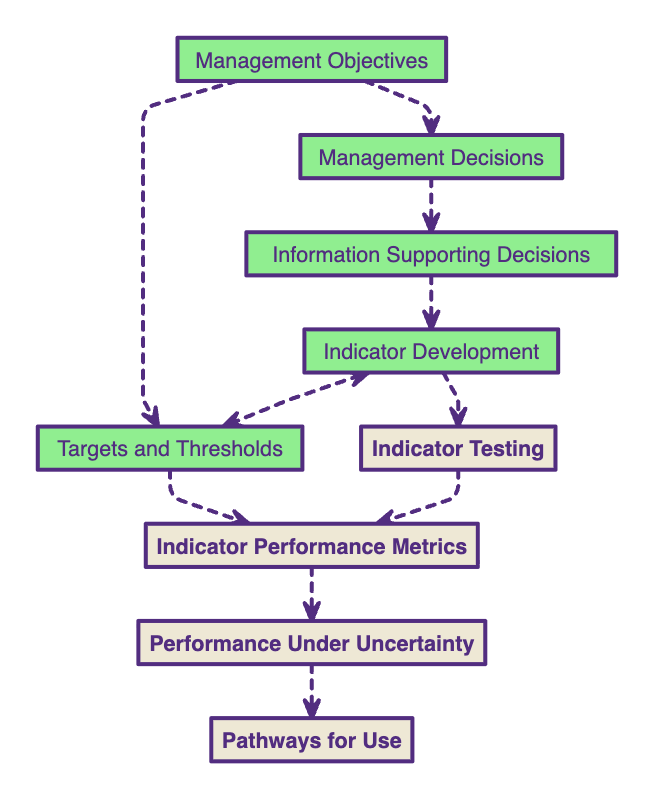
\includegraphics[width=1\linewidth]{MiniWK_Summary_files/figure-latex/projectoutline-1}

\begin{ltbluebox}
\emph{This workshop addressed project goals:}\\
* Review and assess existing indicators and evaluate their utility to
support management objectives\\
* Identify and develop priority ecosystem and habitat indicators,
including associated targets and thresholds as appropriate, and identify
specific pathways for incorporation into Council management processes\\
* Develop operational capability by including students and early career
scientists

\end{ltbluebox}

\end{col}

\end{cols}

\end{document}
